\documentclass[notes=hide,hyperref={dvipdfmx,pdfpagelabels=false}]{beamer}
\title{Einführung in Sage - Einheit 8}
\subtitle{Differentation, Taylorsche Formel, Integration}
\mode<article>
{
  \usepackage{fullpage}
  \usepackage{pgf}
  \usepackage[xetex]{hyperref}
  \setjobnamebeamerversion{beamer}
}

\mode<presentation>
{
  %\usetheme{Frankfurt}
 %\usetheme{My}
  \usetheme{Madrid}
  % or ...
%\usecolortheme{seagull}
  %\setbeamercovered{transparent}
  %\setbeamercovered{dynamic}
  % or whatever (possibly just delete it)
}
\usenavigationsymbolstemplate{}
\usefonttheme{structurebold}
\usepackage{multimedia}
%\usepackage{tikz}
\usepackage{fontspec,xunicode,xltxtra}

%\usepackage{polyglossia}
%\setdefaultlanguage[spelling=new, latesthyphen=true]{german}
%\setsansfont{DejaVu Sans}
%\setsansfont{Verdana}
%\setsansfont{Arial}
%\setromanfont{Linux Libertine O}
%\setsansfont{Linux Biolinum O}

\setbeamertemplate{footline}
{
\leavevmode
%\hbox{\begin{beamercolorbox}[wd=.5\paperwidth,ht=2.5ex,dp=1.125ex,
%leftskip=.3cm plus1fill,rightskip=.3cm]{author in head/foot}%
%    \usebeamerfont{author in head/foot}\insertshortauthor
%  \end{beamercolorbox}%
%  \begin{beamercolorbox}[wd=.5\paperwidth,ht=2.5ex,dp=1.125ex,leftskip=.3cm,
%rightskip=.3cm plus1fil]{title in head/foot}%
%    \usebeamerfont{title in head/foot}\insertshorttitle\hfill

\hfill\insertframenumber  \hspace{3pt}

%\inserttotalframenumber
%\hspace*{2ex}
%  \end{beamercolorbox}}%
  \vskip3pt%
}

\usepackage[ngerman]{babel}
\selectlanguage{ngerman}

%
% math/symbols
%
\usepackage{amssymb}
\usepackage{amsthm}
% \usepackage{latexsym}
\usepackage{amsmath}
%\usepackage{amsxtra} %Weitere Extrasymbole
%\usepackage{empheq} %Gleichungen hervorheben
%\usepackage{bm}
 %\bm{A} Boldface im Mathemodus

\usepackage{cellspace}
\setlength{\cellspacetoplimit}{2pt}
\setlength{\cellspacebottomlimit}{2pt}

%%%%%%%%%%%%%%%%%% Fuer Frames [fragile]-Option verwenden!
%Programm-Listing
%%%%%%%%%%%%%%%%%%
%Listingsumgebung fuer verbatim
%Grauhinterlegeter Text
%Automatischer Zeilenumbruch ist aktiviert
\usepackage{listings}
\definecolor{lgray}{gray}{0.80}
%\lstset{backgroundcolor=\color{lgray}, frame=single, basicstyle=\ttfamily, breaklines=true}
\lstnewenvironment{sage}{\lstset{backgroundcolor=\color{lgray},language=Python, emphstyle=\color{red}, frame=single, basicstyle=\ttfamily, breaklines=true,mathescape =true,escapechar=§}}{}


\usepackage{mydef}
%\usepackage{cmap} % you can search in the pdf for umlauts and ligatures
\usepackage{colonequals} %corrects the definition-symbols \colonequals (besides others)
\title{Einführung in Sage}
%
%\subtitle{Disputation} % (optional)

\author{Jochen Schulz}
% - Use the \inst{?} command only if the authors have different
%   affiliation.

\institute{Georg-August Universit\"at G\"ottingen \pgfimage[height=0.5cm]{../figures/unilogo3}}
% - Use the \inst command only if there are several affiliations.
% - Keep it simple, no one is interested in your street address.

\date{\today}

\subject{Sage}
% This is only inserted into the PDF information catalog. Can be left
% out. 

% If you have a file called "university-logo-filename.xxx", where xxx
% is a graphic format that can be processed by latex or pdflatex,
% resp., then you can add a logo as follows:

%\logo{\pgfimage[height=0.5cm]{figures/unilogo3}}


% Delete this, if you do not want the table of contents to pop up at
% the beginning of each subsection:

\AtBeginSection[]
{
  \begin{frame}<beamer>
    \frametitle{Aufbau}
    \tableofcontents[currentsection,currentsubsection]
  \end{frame}
}

\AtBeginSubsection[]
{
  \begin{frame}<beamer>
    \frametitle{Aufbau}
    \tableofcontents[currentsection,currentsubsection]
  \end{frame}
}



%%%%%%%%%%%%%%%%%%%
%Neue Definitionen
%%%%%%%%%%%%%%%%%%%

%Newcommands
\newcommand{\Fun}[1]{\mathcal{#1}}      %Mathcal fuer Funktoren
\newcommand{\field}[1]{\mathbb{#1}}     %Grundkoerper ?? in mathds

\newcommand{\A}{\field{A}}              %Affines A
\newcommand{\C}{\field{C}}              %Complexes C
\newcommand{\Fp}{\field{F}_{\!p}}       %Endlicher Koerper mit p Elementen
\newcommand{\Fq}{\field{F}_{\!q}}       %Endlicher Koerper mit q Elementen
\newcommand{\Ga}{\field{G}_{a}}         %Add Gruppenschema
\newcommand{\K}{\field{K}}              %Generischer Koerper 
\newcommand{\N}{\field{N}}              %Nat Zahlen
\newcommand{\Pj}{\field{P}}             %Projektives P
\newcommand{\R}{\field{R}} 		%Reelle Zahlen
\newcommand{\Q}{\field{Q}}              %Rationale Zahlen  
\newcommand{\Qt}{\field{H}}             %Quaternionen 
\newcommand{\V}{\field{V}}              %Vektorbuendel V
\newcommand{\Z}{\field{Z}}              %Ganze Zahlen

\newcommand{\fdg}{\;|\;}                 %fuer die gilt

%Operatoren
\DeclareMathOperator{\Abb}{Abb}
%\usepackage{sagetex}

\begin{document}
\lstset{basicstyle={\lstbasicfont\footnotesize}}


\maketitle

\begin{frame}{Aufbau}
\tableofcontents
\end{frame}

%======================================================
\section{Differentation}
%======================================================

\begin{frame}{Ableitungen}
Eine Funktion $f: D \ \rightarrow \mathbb{R}$ heißt {\color{red}  differenzierbar} an
der Stelle $x_0 \in D$, wenn 
\[ \lim_{x \rightarrow x_0} \frac{f(x)-f(x_0)}{x -x_0} \]
existiert. \\
Der Grenzwert wird {\color{red} Ableitung} oder {\color{red} Differentialquotient}
von $f$ an $x_0$ genannt und mit $f\,'(x_0)=f^{\,(1)} (x_0)$ bezeichnet.
\end{frame}


\begin{frame}{Bemerkungen}
\begin{itemize}
\item $f$ {\color{red} differenzierbar} (auf $D$): Wenn $f$ an jeder
Stelle von $D$ differenzierbar ist. 
\item {\color{red} Ableitung} von $f$: $f\,'$ für die gilt $f$ differenzierbar auf $D$.
\item Eine Funktion $f:D \rightarrow \mathbb{R}$ ist an $x_0 \in D$
genau dann differenzierbar, wenn es eine lineare Abbildung
$T:\mathbb{R} \rightarrow \mathbb{R}$ gibt, so dass 
\[ f(x_0+h)=f(x_0) +Th + R(h)h, \quad \lim_{h \rightarrow 0} R(h)=0 \]
gilt ($T$ und $R$ hängen i.A. von $x_0$ ab). 
\item $f$ an $x_0 \in D$ differenzierbar => stetig.
\end{itemize}
\end{frame}

\begin{frame}{Beispiele}
\begin{itemize}
\item $(x^n)'=n x^{n-1}$
\item $(e^x)'=e^x$
\item $(\log(x))'= \frac{1}{x}$, $x>0$
\item $(\sin(x))'=\cos(x)$
\item $(\cos(x))'=-\sin(x)$
\end{itemize}
\end{frame}

\begin{frame}{Landau-Symbol}
Sei $f$ eine Funktion, die auf einem Intervall definiert ist, das $0$
enthält. 
\begin{itemize}
 \item {\color{red} $f(x)=O(x^n)$}: Es gibt eine Kontante $C >0$, so dass
\[  \lim_{x \rightarrow 0} \frac{|f(x)|}{|x|^n} \leq C\]
($f(x)$ geht gegen $0$ mindestens so schnell wie $x^n$)
\item {\color{red} $f(x)=o(x^n)$}: 
\[  
 \lim_{x \rightarrow 0} \frac{|f(x)|}{|x|^n}=0
\]
($f(x)$ geht schneller gegen $0$ als $x^n$)
\end{itemize}


\end{frame}

\begin{frame}{Höhere Ableitungen}
\begin{itemize}
\item \alert{$f$ $n$-mal differenzierbar, $f^{\,(n)}$}: Ist $f:D
\rightarrow \mathbb{R}$ $(n-1)$-mal differenzierbar mit der
$(n-1)$-ten Ableitung $f^{\,(n-1)}$ und ist $f^{\,(n-1)}$ wiederum
differenzierbar.
\item Ist $f$ $n$-mal differenzierbar und ist die $n$-te Ableitung $f^{\,(n)}$
stetig, so heißt $f$ $n$-mal {\color{red} stetig differenzierbar}.
\item $f$ heißt {\color{red} unendlich oft differenzierbar}, wenn $f$ $n$-mal
differenzierbar ist für alle $n\in \mathbb{N}$. 
\end{itemize}
\end{frame}

\begin{frame}[fragile]{Ableitungen in Sage}
\begin{sagein}
diff(<Ausdruck>,x) 
\end{sagein}
wird ein Ausdruck oder eine Funktion nach $x$ abgeleitet. \\
\textbf{Beispiele:}
\begin{sagein}
diff(sin(x),x)
\end{sagein}
\begin{sage}
cos(x)
\end{sage}
\begin{sagein}
diff(x^x,x)
\end{sagein}
\begin{sage}
(log(x) + 1)*x^x
\end{sage}
\end{frame}

\begin{frame}[fragile]{Höhere Ableitungen in Sage}
\begin{sagein}
diff(<Ausdruck>,x1,x2,x3,...)
diff(<Ausdruck>,x,<anzahl>) 
\end{sagein}
Ableitung bzgl. der Unbekannten $x1$, dann der entstehende Ausdruck bzgl. $x2$, etc. 
In der 2ten Form gibt \isage{<anzahl>} die Anzahl der Ableitung bzgl. \isage{x} an.\\
\textbf{Beispiele:} 
\begin{sagein}
_=var('x,y,a'); diff(x^2*y^2+a,x,y)
\end{sagein}
\begin{sage}
4*x*y
\end{sage}
\begin{sagein}
diff(1/x,x,10)
\end{sagein}
\begin{sage}
3628800/x^11
\end{sage}

\end{frame}


\begin{frame}[fragile]{Ableitungen - Beispiele}
\begin{sagein}
f(x) = log(cos(x))
f.diff(); diff(f); diff(f,x,x)
\end{sagein}
\begin{sage}
x |--> -sin(x)/cos(x)
x |--> -sin(x)/cos(x)
x |--> -sin(x)^2/cos(x)^2 - 1
\end{sage}
\begin{sagein}
g(x,y) = sin(x^2+y^2)
g.diff(x,x,y)
\end{sagein}
\begin{sage}
(x, y) |--> -8*x^2*y*cos(x^2 + y^2) - 4*y*sin(x^2 + y^2)
\end{sage}
\end{frame}

\begin{frame}{Differentationsregeln}
Seien $f,g:D \rightarrow \mathbb{R}$ differenzierbare Funktionen und
$x_0 \in D$. Dann gilt
\begin{itemize}
\item \alert{Summe}: $(f+g)'(x_0)=f\,'(x_0)+ g\,'(x_0)$
\item \alert{Produktregel}: \[(f \cdot g)'(x_0) = f\,'(x_0) \cdot g(x_0) + f(x_0)g\,'(x_0)\] 
\item \alert{Quotientenregel}: \[\left(\frac{f}{g}\right)'(x_0) = \frac{f\,'(x_0) g(x_0) - f(x_0)
g'(x_0)}{(g(x_0))^2}\]
falls $g(x_0) \neq 0$ .
\end{itemize}
\end{frame}

\begin{frame}{Differentationsregeln}
\begin{itemize}
\item \alert{Kettenregel}: Seien $f:D_f \rightarrow \mathbb{R}$ und $g:D_g
\rightarrow \mathbb{R}$ mit $f(D_f) \subset D_g$. Ferner seien $f$ an
$x_0 \in D_f$ und $g$ an $y_0=f(x_0)$ differenzierbar. Dann gilt
\[ (g \circ f)(x_0) = g\,'(y_0) \cdot f\,'(x_0).  \]
\item \alert{Leibnizsche Regel}:
\[
(f \cdot g)^{(n)} = \sum_{k=0}^n \binom{n}{k} f^{\,(k)} g^{\,(n-k)}.
\]
\item \alert{Umkehrfunktion $f^{\,-1}$}:
\[(f^{\,-1})' \circ f = \frac{1}{f\,'}.\]
\end{itemize}
\end{frame}

\begin{frame}{Wichtige Sätze}
\begin{Satz}
Ist eine Funktion $f$ an $x_0$ differenzierbar und hat sie ein
lokales Extremum, so gilt $f\,'(x_0)=0$.
\end{Satz}
\begin{Satz}[Mittelwertsatz] 
Sei $f$ eine in dem Intervall $[a,b]$ stetige
und in $(a,b)$ differenzierbare Funktion. Dann gibt es ein $\xi \in
(a,b)$, so dass gilt
\[ \frac{f(b)-f(a)}{b-a}= f\,'(\xi). \]  
\end{Satz}
\begin{Satz}
Eine differenzierbare Funktion auf dem Intervall $I$ ist genau
dann konstant, wenn $f\,'(x)$ auf $I$ identisch verschwindet.
 \end{Satz}
\end{frame}

\begin{frame}{Regel von L'Hospital} 
Seien $f,g: D \rightarrow \mathbb{R}$
differenzierbar, und $g\,'(x) \neq 0$, $x \in D$ und 
{\color{red} $\lim_{x \rightarrow a} f(x) = \lim_{x \rightarrow a} g(x)= 0$}. Dann gilt
\[ \lim_{x \rightarrow a} \frac{f(x)}{g(x)} =  \lim_{x \rightarrow a}
\frac{f\,'(x)}{g\,'(x)}, \]
falls der Limes auf der rechten Seite existiert.

Der Fall $a=\pm\infty$ ist auch erlaubt!

\textbf{Bemerkung}: Die Aussage gilt auch für $\lim_{x \rightarrow a} f(x)=\lim_{x \rightarrow a} g(x)= \infty$ 
\end{frame}


\begin{frame}[fragile]{L'Hospital - Beispiele}
\begin{itemize}
\item Bestimmung von $ \lim_{x \rightarrow \infty} \frac{ln(x)}{x^\alpha}$, $\alpha >0$
\begin{sagein}
var('a');f(x) = log(x); g(x) = x^a
assume(a > 0)
limit(diff(f(x),x)/diff(g(x),x),x=oo)
\end{sagein}
\begin{sage}
  0
\end{sage}
\begin{sagein}
assume(a,'integer')
limit(f(x)/g(x),x=oo)
\end{sagein}
\begin{sage}
  0
\end{sage}
\end{itemize}
\end{frame}


\begin{frame}[fragile]{L'Hospital - Beispiele}
\begin{itemize}
\item Bestimmung von $\lim_{x \rightarrow 0} \frac{\sin(x)}{x}$:
\begin{sagein}
f(x) = sin(x); g(x) = x 
limit(f(x)/g(x), x=0)
\end{sagein}
\begin{sage}
  1
\end{sage}
\begin{sagein}
diff(f(x),x);diff(g(x),x)
\end{sagein}
\begin{sage}
cos(x) 
1
\end{sage}
\begin{sagein}
limit(diff(f(x),x)/diff(g(x),x),x=0)
\end{sagein}
\begin{sage}
1
\end{sage}
\end{itemize}
\end{frame}

%------------------------------------------------------------
\section{Taylorsche Formel}
%-------------------------------------------------------------

\begin{frame}{Taylorsche Formel}
Sei $f:I \rightarrow \mathbb{R}$ $(n+1)$-mal differenzierbar und seien
$x,x_0 \in I$, $x \neq x_0$. Dann gibt es $\xi \in \mathbb{R}$, so
dass
\begin{eqnarray*}
f(x)& = & f(x_0) + \frac{f\,'(x_0)}{1!}(x-x_0)+
\frac{f\,''(x_0)}{2!}(x-x_0)^2\\[0.5cm]
 & & + \cdots + \frac{f^{\,n}(x_0)}{n!}(x-x_0)^n +R_n(x,x_0) 
\end{eqnarray*}
gilt mit dem  {\color{red} Lagrangschen Restglied}
\[ R_n(x,x_0) := \frac{f^{\,(n+1)}(\xi)}{(n+1)!} (x-x_0)^{n+1}. \]
\end{frame}

\begin{frame}[fragile]{Restglied}
Für das Restglied gibt es noch andere Darstellungen:
\begin{itemize}
\item Darstellung von \alert{Cauchy}
\[ R_n(x,x_0)= \frac{f^{\,(n+1)}(\xi)}{n!} (x- \xi)^{n}(x-x_0).\]
\item \alert{Integraldarstellung}
\[ R_n(x,x_0)= \int_{x_0}^x \frac{f^{\,(n+1)}(t)}{n!}  (x-t)^n dt.\]
\end{itemize}
\end{frame}

\begin{frame}{Taylorreihe}
Sei $f:I \rightarrow \mathbb{R}$ unendlich oft  differenzierbar und seien
$x,x_0 \in I$, $x \neq x_0$. Dann nennt man die Reihe
\[ \sum_{n=0}^\infty \frac{f^{\,(n)}(x_0)}{n!}(x-x_0)^n \]
die {\color{red} Taylorreihe} von $f(x)$ um den Entwicklungspunkt
{\color{red} $x_0$}.

\bigskip
Die Taylorreihe stellt die Funktion $f$, wenn das Restglied $R_n(x,x_0)$ für $n
\rightarrow \infty$ gegen $0$ geht.
\end{frame}

\begin{frame}{Hinreichende Bedingungen}
\begin{itemize}
\item Die Funktion $f$ läßt sich auf $I\cap (x_0-\delta, x_0+\delta)$ durch die Taylorreihe darstellen, wenn
\[
\delta:= \frac{1}{\limsup_{n \rightarrow \infty} \sqrt[n]{A_n}}>0
 \]
mit $A_n=\sup_{x \in I}  \frac{|f^{\,(n)}(x)|}{n!}$ gilt.
\item Gibt es ein $M>0$, so dass $|f^{\,(n)}(x)|\leq M^n$ ist für $x \in
I$, $n \in \mathbb{N}$, so läßt sich $f$ auf $I$ durch die Taylorreihe
darstellen.
\item Es gebe ein $M$ mit  $f^{\,(n)}(x)\geq -M^n$, $x \in [a,b]$. Dann
gilt die Taylorreihendarstellung für alle $x \in [a,b]$ mit
$|x-x_0|<b-x$. 
\end{itemize}
\end{frame}

\begin{frame}{Beispiele}
\begin{itemize}
\item Ist $f(x) = \sum_{n=0}^k a_n x^n$ ein Polynom, so gilt für jeden Punkt $x_0 \in \R$
\[
 f(x) = \sum_{n=0}^\infty \frac{f^{\,(n)}(x_0)}{n!}(x-x_0)^n 
 = \sum_{n=0}^k  \frac{f^{\,(n)}(x_0)}{n!}(x-x_0)^n
\]
\end{itemize}
\end{frame}


\begin{frame}{Beispiele}
\begin{itemize}
\item Für $f(x)=\exp(x)$ und $x_0 \in \mathbb{R}$ gilt 
\[ \exp(x)= \sum_{n=0}^\infty \frac{\exp(x_0)}{n!} (x-x_0)^n, \quad x
\in \mathbb{R}.\]
\item Für $f(x)=\log(x)$ und $x_0=1$ gilt
\[ \log (x) = \sum_{n=1}^\infty \frac{(-1)^{n-1}}{n}(x-1)^n, \quad 0 <
x \leq 2.\]
\item Für $f(x)= (1+x)^a$, $a\in \mathbb{R}$  und $x_0=0$ gilt
\[ (1+x)^a= \sum_{n =0}^\infty \binom{a}{n}{x^n}, \quad -1 <
x < 1. \]
\end{itemize}
\end{frame}

\begin{frame}[fragile]{Visualisierung I}
Entwickle $f(x)=exp(x)$ um $x_0=0$. Wir entwickeln gemäß der Taylorformel und erhalten die
Approximationen $g_0(x):=1$, $g_1(x):=1+x$,
$g_2(x):=1+x+\frac{1}{2}x^2$, $g_3(x)=\sum_{i=0}^3 \frac{x^i}{i!}$ und 
$g_4(x)=\sum_{i=0}^4 \frac{x^i}{i!}$.

\begin{sagein}
var('n,k');f(x) = exp(x)
g = [sum(x^k/factorial(k),k,0,n) for n in [0..4]]; g
\end{sagein}
{\color{blue}\[ \left[1, x + 1, \frac{1}{2} \, x^{2} + x + 1, \frac{1}{6} \, x^{3} +
\frac{1}{2} \, x^{2} + x + 1, \frac{1}{24} \, x^{4} + \frac{1}{6} \,
x^{3} + \frac{1}{2} \, x^{2} + x + 1\right]\]}
% \begin{sage}
% [1, x + 1, 1/2*x^2 + x + 1, 1/6*x^3 + 1/2*x^2 + x + 1, 1/24*x^4 +
% 1/6*x^3 + 1/2*x^2 + x + 1]
% \end{sage}
\begin{sagein}
p = plot(f,(-3,2),color='black')
for n in [0..4]:
    p += plot(g[n],(-3,2),rgbcolor=hue(n/5),label=n)
p.show()
\end{sagein}
\end{frame} 

\begin{frame}[fragile]{Visualisierung II}
 \begin{center}
  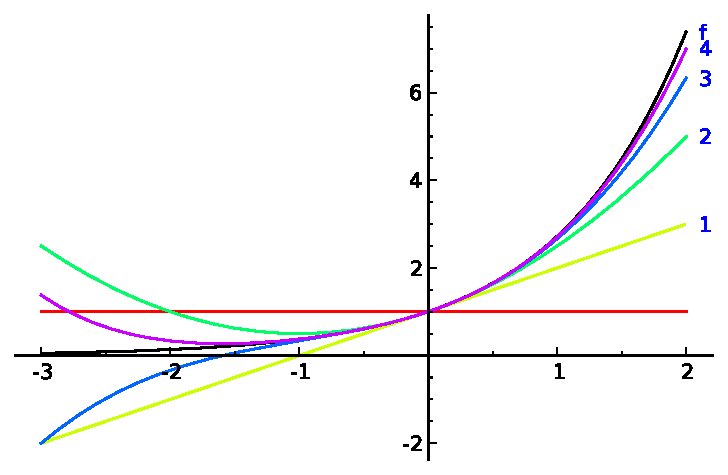
\includegraphics[width=\textwidth]{figures/taylorexp.pdf}
 \end{center}
\end{frame}


\begin{frame}[fragile]{Gegenbeispiel}
Die Funktion
\[ f(x) = \left \{ \begin{array}{ll}
\exp(-1/x^2), & \mbox{ für } x \neq 0\\
0, & \mbox{ für } x = 0\\
\end{array} \right. \]
ist nicht durch ihre Taylorreihe an $x_0=0$ darstellbar. Die Taylorreihe zu $f$
ist identisch $0$, da $f^{\,n}(0)=0$ ist für alle $n \in \mathbb{N}$. \\
\begin{sagein}
plot(exp(-1/x^2),(-0.5,0.5)) 
\end{sagein}
\begin{center}
  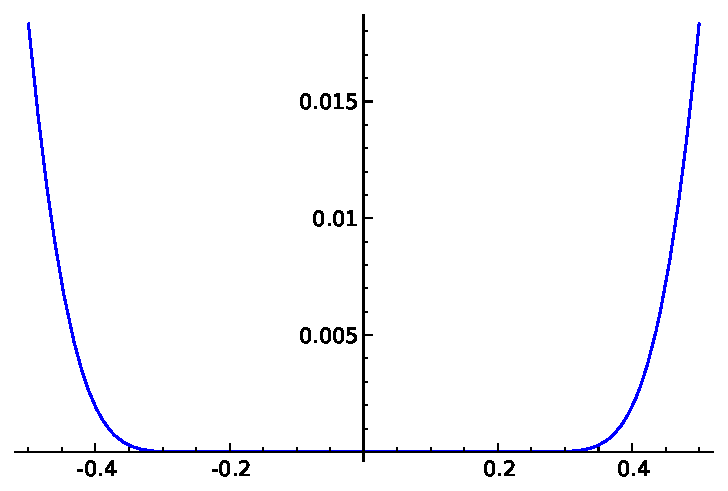
\includegraphics[height=4cm]{figures/taylorgegen.pdf}
 \end{center}
\end{frame}

\begin{frame}[fragile]{Taylorformel in Sage}
\begin{sagein}
taylor(f, x, x0, n)
\end{sagein}
Taylorpolynom $(n-1)$-ten Grades zu einem Ausdruck $f$ 
(mit Unbekannten $x$) am Entwicklungspunkt $x0$. \\
\textbf{Beispiele}:
\begin{sagein}
taylor(1/(1-x),x,0,5)
\end{sagein}
{\color{blue}\[ x^{5} + x^{4} + x^{3} + x^{2} + x + 1\]}
\begin{sagein}
taylor(sin(x),x,2,5)
\end{sagein}
{\small\color{blue}\[ \frac{1}{24} \, {\left(x - 2\right)}^{4} \sin\left(2\right) -
\frac{1}{6} \, {\left(x - 2\right)}^{3} \cos\left(2\right) - \frac{1}{2}
\, {\left(x - 2\right)}^{2} \sin\left(2\right) + {\left(x - 2\right)}
\cos\left(2\right) + \sin\left(2\right)\]}
\end{frame}

% \begin{frame}[fragile]{Bemerkungen}
% \begin{itemize}
% \item Das in den Darstellungen auftretende Symbol \isage{O} ist das
%                Landau-Symbol. Mit ihm kann man in MuPAD rechnen. 
% \begin{sagein}
% o1:=O(x^2): o2:=O(x^3):
% o1*o2, o1+o2, o1/o2
% \end{sagein}
% \begin{sage}
%      5      2    / 1 \
%   O(x ), O(x ), O| - |
%                  \ x /
% \end{sage}
% \end{itemize}
% \end{frame}

% \begin{frame}[fragile]{Bemerkungen}
% \begin{itemize}
% \item Man kann mit den  Objekten des Typs  \isage{Series::Puiseux}
%              rechnen, insofern sie denselben Entwicklungspunkt haben. Z. B., können sie addiert oder
%              multipliziert werden.
% \begin{sagein}
% taylor1+taylor2
% \end{sagein}
% \begin{small}
% \begin{sage}
%   Error: different series variables or 
%    expansion points [Series::Puiseux::plus] 
% \end{sage}
% \end{small}
% \begin{sagein}
% taylor3:=taylor(exp(x),x=2,5):
% taylor2*taylor3
% \end{sagein}
% \begin{scriptsize}
% \begin{sage}
%                                                     2        3 
%       2          2                2       2  4 exp(2)  (x - 2) 
% exp(2) + 2 exp(2)(x - 2) + 2exp(2) (x - 2) + -----------------  
%                                                      3  
%            2        4 
%    2 exp(2)  (x - 2)             5 
%  + ------------------ + O((x - 2) ) 
%             3 
% \end{sage}
% \end{scriptsize}
% \end{itemize}
% \end{frame}

%-------------------------------------------------
\section{Integration}
%------------------------------------------------

\begin{frame}{Begriffe I}
\begin{itemize}
\item  Sei $[a,b]$ ein Intervall. Gilt $a=a_0 < a_1 <a_2 < \dots <
                                 a_n=b$, so nennt man $Z=(a_0, \dots
                                 ,a_n)$ eine {\color{red} Zerlegung} von
                                 $[a,b]$.
\item Eine Funktion $\phi:[a,b] \rightarrow \mathbb{R}$ heißt {\color{red}
                                 Treppenfunktion}, wenn es eine
                                 Zerlegung $Z$ von $[a,b]$ gibt, so dass
                                 $\phi$ konstant ist auf jedem
                                 Teilintervall $(a_i,a_{i+1})$ von $Z$.
\item Wir erklären das Integral einer Treppenfunktion $\phi$ durch
\[\int_Z \phi := \sum_{k=1}^n c_k (a_k -a_{k-1}).\]
Dabei ist $Z$ die zugehörige Zerlegung und $c_k=\phi(x)$, $x\in
(a_{k-1},a_k)$.  
\item Die Menge aller Treppenfunktionen auf $[a,b]$ sei $T[a,b]$.
\end{itemize}
\end{frame}

\begin{frame}[fragile]{Begriffe II}
Für eine beschränkte Funktion $f[a,b]\rightarrow \mathbb{R}$
heißt
\[ \int^*f:= \inf  \{ \int \psi \ | \ \psi \in T[a,b], f \leq \psi \}. \]
das {\color{red} Oberintegral} und 
\[ \int_*f:= \sup  \{ \int \psi \ | \ \psi \in T[a,b], f \geq \psi \}.\]
das {\color{red} Unterintegral}. Es gilt für $\phi, \psi \in T[a,b]$ mit
$\phi \leq f \leq \psi$ die Ungleichung
\[ \int \phi \leq \int_* f \leq \int^* f \leq \int \psi.\]
\end{frame}

\begin{frame}[fragile]{Visualisierung in Sage}
\begin{sagein}
f = Piecewise([[(-pi,0),(cos(x)).function(x)]])
rsf = f.riemann_sum(10,mode="midpoint")
P = f.plot(rgbcolor=(0.7,0.1,0.5), plot_points=40)
Q = rsf.plot(rgbcolor=(0.7,0.6,0.6), plot_points=40)
L = add([line([[b,0],[b,f(x=b)]],rgbcolor=(0.7,0.6,0.6))+line([[a,0],[a,f(x=a)]],rgbcolor=(0.7,0.6,0.6)) for (a,b),f in rsf.list()])
(P + Q +L)
\end{sagein}
\begin{center}
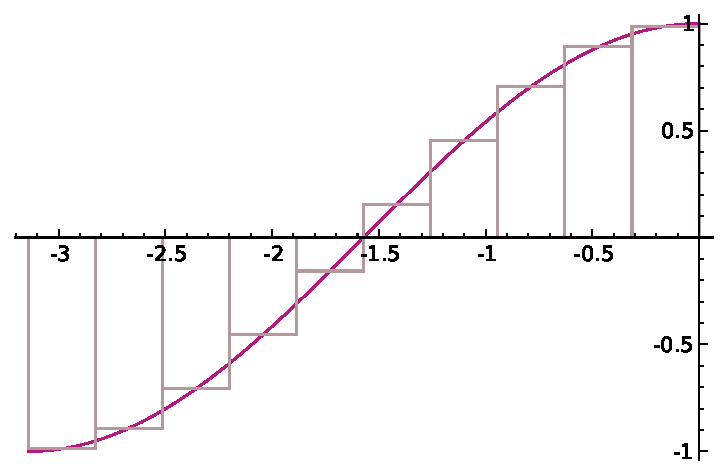
\includegraphics[width=6cm]{figures/riemann.pdf}
\end{center}
\end{frame}

% \begin{frame}[fragile]{Visualiserung mit MuPAD II}
% \begin{sagein}
% p:=student::plotRiemann(cos(x),x=-PI..PI,30): 
% plot(p)
% \end{sagein}
% \begin{center}
% %\includegraphics[width=8cm]{figures/riemann1.png}
% \end{center}
% \end{frame} 

\begin{frame}{Das Riemannsche Integral}
Eine beschränkte Funktion $f:[a,b] \rightarrow \mathbb{R}$ heißt {\color{red}
integrierbar}, wenn Ober- und Unterintegral von $f$ auf $[a,b]$ übereinstimmen.\\
Der gemeinsame Wert heißt das {\color{red} Integral} von $f$ und wird mit 
\[ \int_a^b f(x)dx \]
bezeichnet.\\ 
($f$ der Integrand, $x$ Integrationsvariable, $a$, $b$ Integrationsgrenzen).
\end{frame}

\begin{frame}{Eigenschaften}
\begin{itemize}
\item Linearität
\[ \int_a^b (\alpha f + \beta g) dx = \alpha \int_a^b fdx + \beta
\int_a^b g dx \]
\item Monotonie
\[  f \leq g \quad \Rightarrow \quad \int_a^b f dx \leq \int_a^b g
dx.\]
\item Ist $f,g$ integrierbar, so auch $f+g$, $f*g$, $f-g$,
$\max\{f,g\}$, $\min \{f,g \}$. 
\end{itemize}
\end{frame}

\begin{frame}{Wichtige Sätze}
\begin{itemize}
\item {\color{red} Stammfunktion} $F$: Ist $f$ stetig auf einem Intervall $I$ und $a \in I$, so ist 
\[F(x)= \int_a^x f(t) dt, x \in I \] eine differenzierbare Funktion mit
$F\,'(x)=f(x)$. 
\item \alert{Unbestimmtes Integral}: alternative Notation für eine Stammfunktion $F$:  $\int f(x) dx$ 
\item Ist $f$ stetig auf $[a,b]$, so gibt es ein $\xi \in [a,b]$ mit
\[\int_a^b f(x)dx = f(\xi) (b-a)\]
\end{itemize}
\end{frame}

\begin{frame}[fragile]{Integrieren in Sage}
\begin{itemize}
 \item Bestimmte Integrale der Form $\int_a^b f(x) dx$
\begin{sagein}
integrate(f,x,a,b) 
\end{sagein}
Dabei ist \isage{f} ein Ausdruck.
\item Unbestimmte Integrale:
\begin{sagein}
integrate(f,x)
\end{sagein}
\item Numerische Approximationen:
\begin{sagein}
numerical_integral(f,a,b) 
\end{sagein}
(benutzt die GSL-library). 
\end{itemize}
\end{frame}

\begin{frame}[fragile]{Integrieren - Beispiele I}
\begin{sagein}
 integrate(sin(x),x,0,6)
\end{sagein}
\begin{sage}
-cos(6) + 1
\end{sage}
\begin{sagein}
integrate(exp(x)*x,x,2,3),integrate(exp(x)*x,x)
\end{sagein}
{\color{blue}\[\left(-e^{2} + 2 \, e^{3}, {\left(x - 1\right)} e^{x}\right)\]}
% \begin{sage}
% -e^2 + 2*e^3
% \end{sage}
\begin{sagein}
integrate(1/x^2,x,1,oo)
\end{sagein}
\begin{sage}
  1
\end{sage}
\begin{sagein}
numerical_integral(sin(1/x)*x,1,2)
\end{sagein}
\begin{sage}
  (0.91905916759870254, 1.0203606488609102e-14)
\end{sage}
\end{frame}


\begin{frame}[fragile]{Integrieren - Beispiele II}
\begin{sagein}
assume(a<>-1)
integrate(x^a*b,x)
\end{sagein}
{\color{blue} \[ \frac{b x^{{\left(a + 1\right)}}}{a + 1}\]}
% \begin{sage}
% b*x^(a + 1)/(a + 1)
% \end{sage}
\begin{sagein}
forget();a=-1
integrate(x^a*b,x)
\end{sagein}
{\color{blue} \[ b \log\left(x\right)\]}
% \begin{sage}
%  b*log(x)
% \end{sage}
\end{frame}

\begin{frame}{Uneigentliche Integrale}
Sei $f$ auf $[a,b)$ erklärt (eventuell $b=\infty$) und sei $f$ auf jedem
abgeschlossenen Teilintervall integrierbar. Man definiert
\[  \int_a^b f(x)dx := \lim_{z \rightarrow b (-0)} \int_a^z f(x)dx,\]
falls der Limes existiert. Man spricht von einem {\color{red}
uneigentlichen Integral}.
\end{frame}

\begin{frame}{Funktionenfolgen}
\begin{itemize}
\item Sei $(f_n)_n$ eine Folge integrierbarer Funktionen auf
$[a,b]$. Konvergiert $(f_n)_n$ gleichmäßig, so ist die Grenzfunktion
integrierbar mit
\[ \int_a^b \lim_{n \rightarrow \infty} f_n(x) dx = \lim_{n
\rightarrow \infty} \int_a^b f_n(x) dx .\]
\item Sei $(f_n)_n$ eine Folge differenzierbarer Funktionen auf
$[a,b]$. $(f\,'_n)_n$ konvergiere gleichmäßig und es existiere ein $x_0
\in [a,b]$ für den $f_n(x_0)$ konvergiert. Dann konvergiert $(f_n)_n$
gleichmäßig mit $( \lim_{n \rightarrow \infty} f_n(x))' = \lim_{n
\rightarrow \infty} f\,'_n(x)$.  
\end{itemize}
\end{frame}

% 

% \end{frame}
% 
% \begin{frame}[fragile]{Nützliches}
% \begin{itemize}

% \item Durch Voranstellen von {\color{blue}\isage{!}} kann man UNIX-Befehle innerhalb
% MuPAD aufrufen. Zum Beispiel kann man sich den Inhalt des aktuellen
% Verzeichnisses durch {\color{blue} \isage{!ls}} anzeigen lassen.
% \end{itemize}
% \end{frame}
\end{document}
